% begin module infinite-limit-at-infinity-ex8
\begin{frame}
\begin{example}%[Example 8, p. 236]
\begin{columns}[c]
\column{.5\textwidth}
\psset{xunit=0.8cm, yunit=0.8cm}
\begin{pspicture}(-3.2,-3.5)(3.2,3.7)
\psframe*[linecolor=white](-3.2,-3.5)(3.2,3.7)
\psaxes[ticks=none, labels=none]{<->}(0,0)(-3,-3.5)(3,3.5)
\fcLabelXOne
\fcLabelYOne
%Function formula: (x)^{3}
\psplot[linecolor=red, plotpoints=1000]{-1.5}{1.5}{x 3 exp }
\rput[l] (1.5, 1){\footnotesize $y=x^3$}
\end{pspicture}
%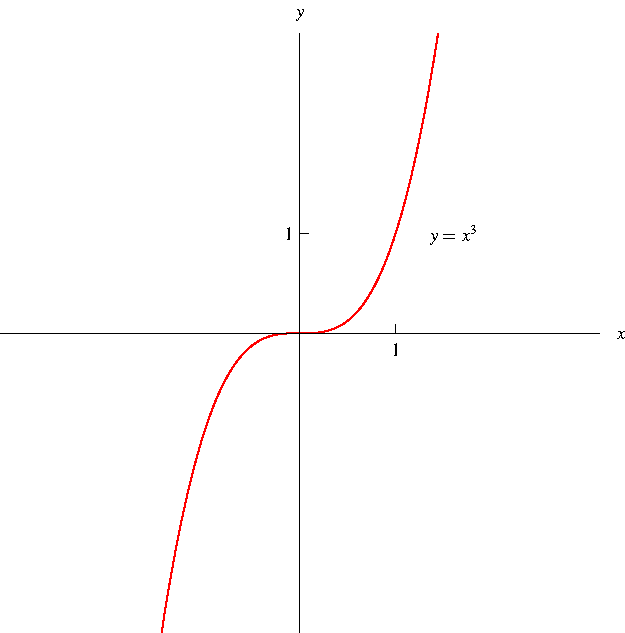
\includegraphics[width=5cm]{curve-sketching/pictures/01-02-xcubed.pdf}
\uncover<2->{%
\abovedisplayskip=0pt
\belowdisplayskip=0pt
\[
10^3  =  1000, \qquad  100^3  =  1,000,000,
\]
\abovedisplayskip=0pt
\belowdisplayskip=0pt
\[
1000^3 = 1,000,000,000
\]
}%
\column{.5\textwidth}
Find $\lim_{x\to\infty} x^3$ and $\lim_{x\to -\infty} x^3$.
\begin{itemize}
\item<2->  When $x$ is large, so is $x^3$.
\item<3->  By taking $x$ large enough, we can make $x^3$ as large as we like.
\item<4->  Therefore $\lim_{x\to \infty} x^3 = \infty$.
\item<5->  Similarly, $\lim_{x\to -\infty} x^3 = -\infty$.
\end{itemize}
\end{columns}
\end{example}
\end{frame}
% end module infinite-limit-at-infinity-ex8
